\mytitle{À Luz de Caravaggio} % Título do Artigo    
\addchaptersummary{À Luz de Caravaggio}{Sumario/Figs_Sumario/FigArtigo2.jpg}{Nesse artigo, a vida de Michelangelo Merisi, Caravaggio, é apresentada por meio de suas obras, e essas interpretadas pelos olhos da Óptica Geométrica.}{Milena Camila Fernandes} 
\newcommand{\artigodois}{\begin{center}\textcolor{base}{\MakeUppercase{À Luz de Caravaggio}}\end{center}}

\begin{multicols}{2}

Apresentar Michelangelo Merisi da Caravaggio (Caravaggio, 29 de setembro de 1571 — Porto Ercole, 18 de julho de 1610) \ref{ref1:artigo2} não é tarefa simples, tanto pela complexidade da arte quanto do próprio artista. Para isso, ele será retratado aqui por meio dos seus quadros e contextos\footnote{Por muitas vezes, a adjetivação e interpretação de Caravaggio e suas obras presentes nesse artigo --- quando não acompanhadas de fontes científicas --- são feitas através dos olhos da autora do texto, uma simples admiradora de seu trabalho.}. 

\begin{figure}[H]
	\centering
	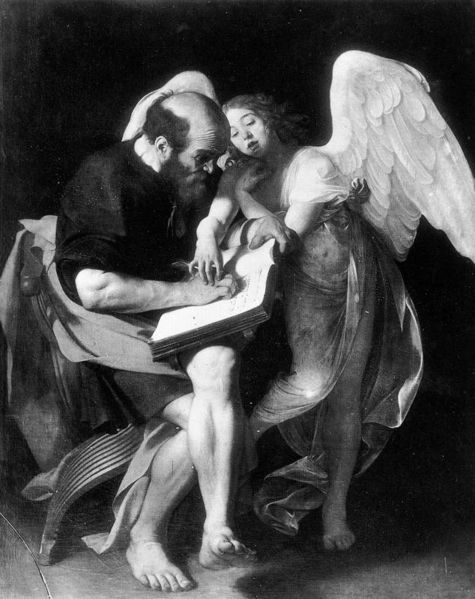
\includegraphics[width=0.9\linewidth]{Figuras/Artigo2/m1.jpg}
	\protect\caption{São Mateus e o Anjo. Caravaggio; c. 1602; Óleo sobre tela; 295 cm; (destruído). [Fonte: \href{https://www.wikiart.org/pt/caravaggio}{WikiArt}].}
	\label{fig:m1}
\end{figure}

Como início, podemos mostrar esse maneirista de formação, mas considerado o pai da arte barroca, por meio de duas obras, as quais  tinham o mesmo objetivo: retratar o apóstolo São Mateus e o Anjo para serem colocados na Capela Contarelli da Igreja de São Luís dos Franceses (Roma). A primeira versão da obra (Figura \ref{fig:m1}) foi rejeitada pelos cardeais, isso porque, como podemos notar, a pintura de Caravaggio traz uma proximidade extremamente humana entre o homem e o Anjo, retratando ambos em igualdade, em que o Anjo chega a segurar a mão de São Mateus para o ajudar. Assim, Caravaggio deixa sua essência nessa obra — uma retratação sem idealizações —, mas que seguia o caminho oposto desejado pelos cardeais, tornando-a ``humana demais''  \reftres{ref1:artigo2}{ref2:artigo2}{ref3:artigo2}. Segundo o cardeal Matteo Contarelli, a obra deveria seguir os seguintes requisitos \ref{ref4:artigo2}: 

\textit{``San Matteo na cadeira com um livro, ou volume, como melhor pareça, no qual mostre a escrita ou a vontade de escrever o Evangelho e ao lado dele o Anjo de pé maior do que o natural em acto que pareça de pensar ou noutra atitude.''}

Desse modo, Caravaggio teve que a refazer e o resultado pode ser visto na Figura \ref{fig:m2}. É notável a diferença de proximidade entre o Anjo e São Mateus, dando ao primeiro a santidade necessária exigida pela Igreja, como um ser que desce para fornecer ao humano a inspiração para dar início a sua escrita sagrada, mas que mantém uma distância que caracteriza sua hierarquia, sua importância divida. Essa obra se encontra na \href{https://commons.wikimedia.org/wiki/File:1475RomaSLuigiFrancesiInside.jpg}{capela} até os dias atuais, mas a primeira versão foi destruída num incêndio no final da Segunda Guerra Mundial, restando apenas uma foto da pintura, exibida nesse artigo.

Apesar de ambas as obras terem diferenças em diversos aspectos entre os personagens que as compõem, é certo que elas usam uma técnica em comum: a luz e sombra. Essa técnica já existia na história da arte, mas foi aperfeiçoada por Caravaggio, dando-a um caráter singular: \textbf{o tenebrismo}. Ela consiste em um claro-escuro ainda mais extremado e dramático, em que o uso da luz e sombra é construído para trazer à imagem um realismo psicológico, um estado de espírito que ultrapassa o quadro e atinge nossos sentidos \refdois{ref1:artigo2}{ref7:artigo2}.

\begin{figure}[H]
	\centering
	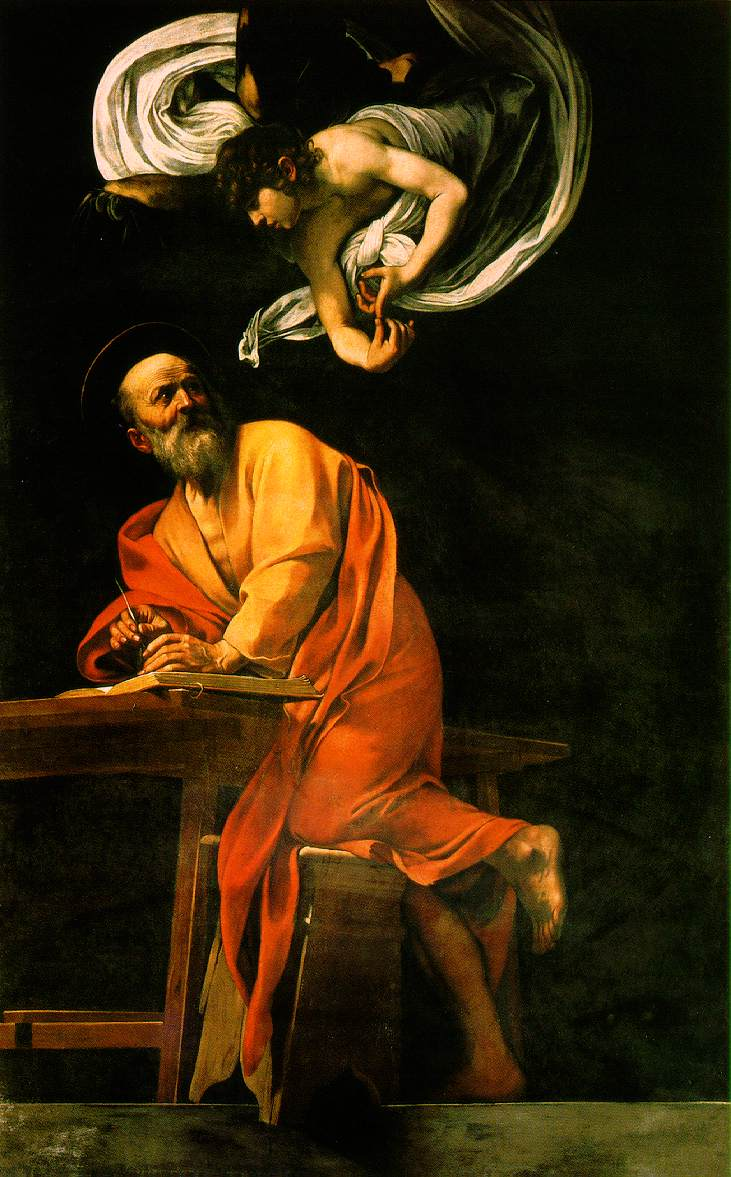
\includegraphics[width=0.8\linewidth]{Figuras/Artigo2/m2.jpg}
	\protect\caption{A Inspiração de São Mateus. Caravaggio; c. 1602; Óleo sobre tela; 292 cm × 186 cm; San Luigi dei Francesi, Roma. [Fonte: \href{https://www.wikiart.org/pt/caravaggio}{WikiArt}].}
	\label{fig:m2}
\end{figure}

Nesse viés, escuros profundos ao fundo na tela complementam uma luz extremamente vívida em pontos  estratégicos — como nos rostos, iluminando a expressão dos personagens ou evidenciando algum movimento, como se um refletor estivesse acima da figura \ref{ref1:artigo2}. Tais pontos foram milimetricamente concebidos para que os detalhes nos saltassem os olhos e transmitissem algum tipo de sentimento.  
	
A segunda versão da ``A Inspiração de São Mateu'' está na Capela Contarelli, com mais duas obras de Caravaggio que seguem a mesma técnica e temática. À esquerda dessa obra, encontra-se ``O Chamado de São Mateus'' (Figura \ref{fig:m3}) e, ao observá-la, podemos perceber uma fonte de luz que entra pela janela e toca em pontos importantes da tela. A mão de Jesus é meticulosamente iluminada e faz luz a seu movimento, apontando para São Mateus. Esse também tem sua expressão com muita luz — e, em conjunto, a sua mão —, para que seja possível enxergar os detalhes psicológicos que a tela tem a transmitir, como esse gesto simbólico que, segundo o Professor Giovanni Bagnoli ``[...] transforma o pecador em apóstolo [...]'' \refdois{ref2:artigo2}{ref3:artigo2}.
A obra continua com um fundo escuro e com ausência de luz em personagens ``secundários''\footnote{A palavra ``secundários'' foi utilizada para denotar os personagens que estão para além do significado religioso que ela deveria ter, como por exemplo o homem que conta moedas, ao canto da mesa, o qual foi considerado um autorretrato de Caravaggio.} do cenário, como no rosto de Pedro, que segura Jesus, em que apenas a sua mão tem maior enfoque. 

Para completar a tríade de uma parte da Capela, temos ``O Martírio de São Mateus'' (Figura \ref{fig:m4}), obra à direita da ``Inspiração de São Mateus''. Nesse trabalho, podemos ver um carrasco no centro da composição, com o apóstolo Mateus deitado. No entorno, existem muitas figuras expressivas típicas do barroco\footnote{Na pintura, escultura, arquitetura e artes decorativas, estilo, com elementos do alto Renascimento e do Maneirismo e ligado à estética da Contrarreforma, nascido em Roma c1600 e cujas características básicas são o dinamismo do movimento com o triunfo da linha curva e (esp. na escultura e pintura) a busca da captação das reações emocionais humanas. Cedo internacionalizado, o estilo ganhou traços específicos em cada país \ref{ref6:artigo2}.}. Nessa situação, a luz dá foco ao movimento dos dois personagens ``principais'', à movimentação do carrasco que dará um golpe fatal no apóstolo e à proteção que São Mateus tenta manter com um gesto de defesa\footnote{Nessa obra, é comprovado que o homem no fundo da tela, olhando diretamente para ``nós'', é um autorretrato de Caravaggio.}.

Olhando o tenebrismo pelo viés da Física, podemos entender melhor como usar o claro-escuro pela compreensão de alguns conceitos da óptica geométrica no que se refere ao que é luz, sombra e penumbra. Inicialmente, a fonte de luz que incidirá sobre o objeto pode ser de origem primária --- gera sua própria luz, como o Sol ---, ou de origem secundária, que necessita que uma fonte de luz primária reflita no objeto para que ele seja visto, como a Lua. Uma vez que a fonte emite luz, ela pode encontrar um objeto que é opaco, transparente ou translúcido. Para o primeiro, a luz é absorvida e refletida e não é possível que ela o atravesse. Já o segundo é um objeto que permite a passagem de luz sem que ela sofra desvios e, por fim, no terceiro caso é permitida a passagem de luz, mas ela sofre desvios e o observador não consegue enxergar a imagem com nitidez. 

\end{multicols}

\begin{figure}[H]
    \centering
	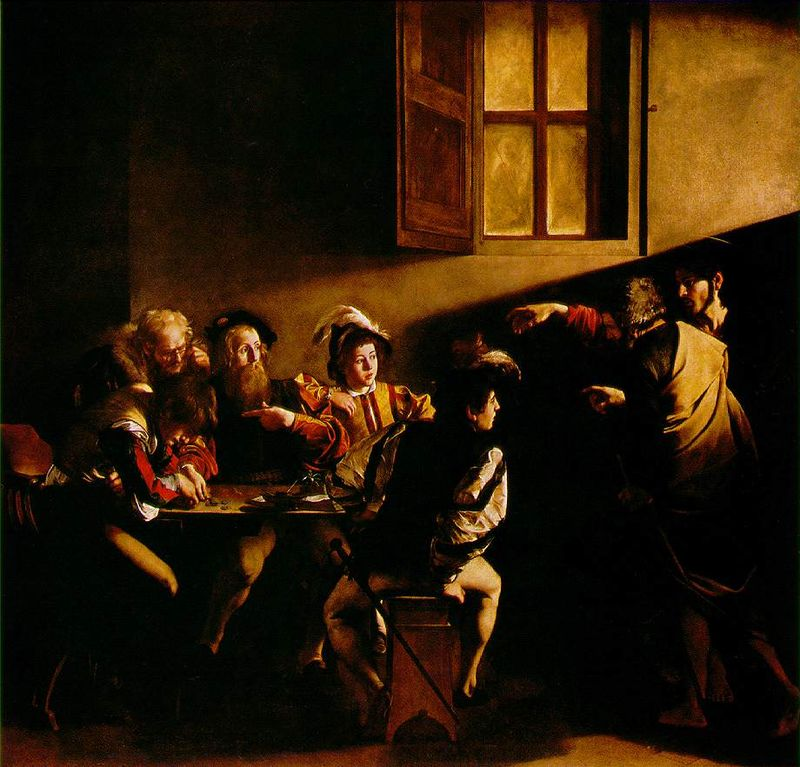
\includegraphics[width=0.7\linewidth]{Figuras/Artigo2/m9.jpg}
	\protect\caption{Vocação de São Mateus. Caravaggio; c. 1599-1600; Óleo sobre tela; 340 cm × 322 cm; San Luigi dei Francesi, Roma. [Fonte: \href{https://www.wikiart.org/pt/caravaggio}{WikiArt}].}
    \label{fig:m3}
\end{figure}

\begin{multicols}{2}


Paralelo a isso, a junção da fonte, objeto e anteparo (ou observador) obedecerá o Princípio da Propagação Retilínea da Luz\footnote{O Princípio da Independência dos Raios Luminosos e o Princípio da Reversibilidade dos Raios Luminosos também se fazem presente nos conceitos de luz e sombra, mas não foram abordados neste artigo. Todos podem ser melhor compreendidos em \ref{ref4:artigo2}.}, isto é, a luz se propaga em linha reta nos meios homogêneos, transparentes e isotrópicos. Como consequência, temos a produção de sombra (ausência total de luz) atrás de objetos opacos, para os casos em que a fonte é puntiforme, e também a produção de sombra e penumbra (ausência parcial de luz) quando a fonte é extensa \refdois{ref8:artigo2}{ref9:artigo2}.

Nas obras apresentadas neste artigo, é possível identificar que as técnicas utilizadas seguem os preceitos apresentados acima. Na Figura \ref{fig:m2}, a luz incide acima (e lateralmente) de São Mateus e produz sombra em lugares nos quais ela previamente encontrou um objeto que a absorveu e refletiu. Isso pode ser observado, por exemplo, abaixo do apóstolo, nos detalhes do seu pé, nas dobras de suas vestimentas e no peito do Anjo. Em conjunto, é possível notar que, em cada detalhe da tela os princípios são respeitados, como o da trajetória retilínea da luz nas curvaturas dos braços do Anjo. 
\end{multicols}

\begin{figure}[H]
	\centering
	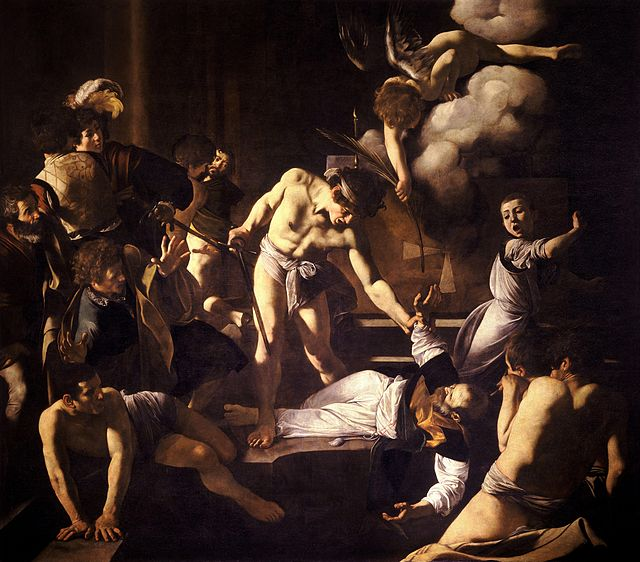
\includegraphics[width=0.7\linewidth]{Figuras/Artigo2/m7.jpg}
	\protect\caption{O Martírio de São Mateus. Caravaggio; c. 1599-1600; Óleo sobre tela; 323 cm × 343 cm ; San Luigi dei Francesi, Roma. [Fonte: \href{https://www.wikiart.org/pt/caravaggio}{WikiArt}].}
	\label{fig:m4}
\end{figure}

\begin{multicols}{2}
    
O mesmo ocorre com as Figuras \ref{fig:m3} e \ref{fig:m4}. Na primeira, vale ressaltar o enfoque que o Caravaggio dá às mãos de Jesus, Pedro e Mateus, evidenciando o objetivo da cena. Já na segunda, é nítida a percepção dos dois elementos centrais da tela, iluminados por uma fonte lateral que permite que as expressões do carrasco e de São Mateus sejam evidenciadas, mesmo que seus rostos não estejam totalmente visíveis. 
	
A três obras apresentadas aqui ainda estão expostas na Capela Contarelli, como apresentado na Figura \ref{fig:m5}. Essas e outras várias do artista fazem uso do tenebrismo, técnica que revolucionou o teatro, o cinema, a pintura e a fotografia. Até os dias atuais, sua influência no uso da luz e sombra se faz presente em todas essas expressões artísticas\footnote{E certamente em muitas outras que não foram citadas aqui.}. 
	
É evidente que, com a morte de Michelangelo Merisi, com apenas 38 anos, a história da arte perdeu um de seus maiores gênios que concedeu à humanidade uma coleção de obras monumentais, em tamanho e expressividade, que nunca deixarão de ter influência na arte e todos os seus vieses. Seu divino claro-escuro o faz eternamente vivo. 

\begin{figure}[H]
	\centering
	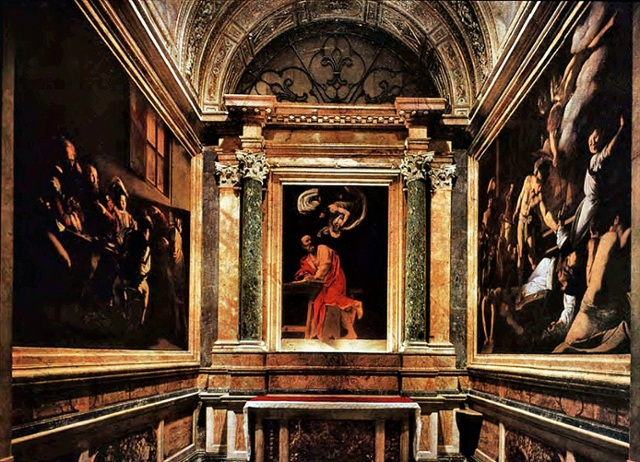
\includegraphics[width=0.95\linewidth]{Figuras/Artigo2/m8.jpg}
	\protect\caption{Capela Contarelli da igreja de S. Luís dos Franceses, em Roma, com as três pinturas de Caravaggio. [Fonte: \href{https://pt.wikipedia.org/wiki/A_Inspira\%C3\%A7\%C3\%A3o\_de\_S\%C3\%A3o\_Mateus\#/media/Ficheiro:1475RomaSLuigiFrancesiInside.jpg}{WikiArt}].}
	\label{fig:m5}
\end{figure}

\noindent\textit{``Não sou um pintor valentão, como me chamam, mas sim um pintor valente, isto é, que sabe pintar bem e imitar bem as coisas naturais.''}\\
	Michelangelo Merisi, dito Caravaggio.

\authorinfo{Milena Camila Fernandes}{http://lattes.cnpq.br/3118223351391736}

\end{multicols}

